% xelatex
\documentclass[letterpaper,
		%twocolumn,
		10pt]{article}
\usepackage[utf8]{inputenc}
\usepackage{metalogo}
\usepackage{xifthen}
\usepackage[colorlinks=true,urlcolor=Blue]{hyperref}
\usepackage{graphicx}
\usepackage{fontspec}
\usepackage[T1]{fontenc}
\usepackage[dvipsnames]{xcolor}
\usepackage{titlesec}
\usepackage[margin=1in]{geometry}
\usepackage{titling}
\newfontfamily\cfont{Noto Sans CJK SC}
\usepackage{libertine}

% Macro to allow image links in XeLaTeX
\ifxetex
  \usepackage{letltxmacro}
  \setlength{\XeTeXLinkMargin}{1pt}
  \LetLtxMacro\SavedIncludeGraphics\includegraphics
  \def\includegraphics#1#{% #1 catches optional stuff (star/opt. arg.)
    \IncludeGraphicsAux{#1}%
  }%
  \newcommand*{\IncludeGraphicsAux}[2]{%
    \XeTeXLinkBox{%
      \SavedIncludeGraphics#1{#2}%
    }%
  }%
\fi
%%%%%%%

% Bold contents of a link
\let\oldhref\href
\renewcommand{\href}[3][blue]{\oldhref{#2}{\color{#1}{#3}}}

% Your name goes here:
\author{Mateus Melo}

% Update date set to last compile:
\date{\today}

% Custom title command.
\renewcommand{\maketitle}{
	\hspace{.25\textwidth}
	\begin{minipage}[t]{.5\textwidth}
\par{\centering{\Huge  \bfseries{\theauthor}}\par}
	\end{minipage}
	\begin{minipage}[t]{.25\textwidth}
{\footnotesize\hfill{}\color{gray}
\hfill{}Download this document:

\hfill{}\href[gray]{https://mateusmelo.xyz/cv.pdf}{https://mateusmelo.xyz/cv.pdf \pdf}

\hfill{}(Last updated \thedate.)
}
	\end{minipage}
}



% Setting the font I want:
\renewcommand{\familydefault}{\sfdefault}
\usepackage{sqrcaps}

% Making the \entry command
\newcommand{\entry}[4]{
\ifthenelse{\isempty{#3}}
{\slimentry{#1}{#2}}{

\begin{minipage}[t]{.15\linewidth}
\hfill \textsc{#1}
\end{minipage}
\hfill\vline\hfill
\begin{minipage}[t]{.80\linewidth}
{\bf#2}\\\textit{#3} \footnotesize{#4}
\end{minipage}\\
\vspace{.2cm}
}}

\newcommand{\slimentry}[2]{

\begin{minipage}[t]{.15\linewidth}
\hfill \textsc{#1}
\end{minipage}
\hfill\vline\hfill
\begin{minipage}[t]{.80\linewidth}
#2
\end{minipage}\\
\vspace{.25cm}
}% end \entry command definition

% Some macros because I'm lazy:
\newcommand{\ufpe}{Universidade Federal de Pernambuco}
\newcommand{\ifpe}{Instituto Federal de Pernambuco}
\newcommand{\acc}{Accenture}
\newcommand{\euro}{Euromercantil}
\newcommand{\life}{Liferay}

% Macros for people's names including link to their websites
%template: \newcommand{\some}{\href{http://generic.com}{Someone}}

\let\lineheight\baselineskip

% Link images
\newcommand{\pdf}{\includegraphics[height=.85em]{cv/pdf.png}}
\newcommand{\yt}{\includegraphics[height=.85em]{cv/yt.png}}
\newcommand{\gh}{\includegraphics[height=.85em]{cv/gh.png}}
\newcommand{\www}{\includegraphics[height=.85em]{cv/www.png}}
\newcommand{\email}{\includegraphics[height=.85em]{cv/email.png}}
\newcommand{\loc}{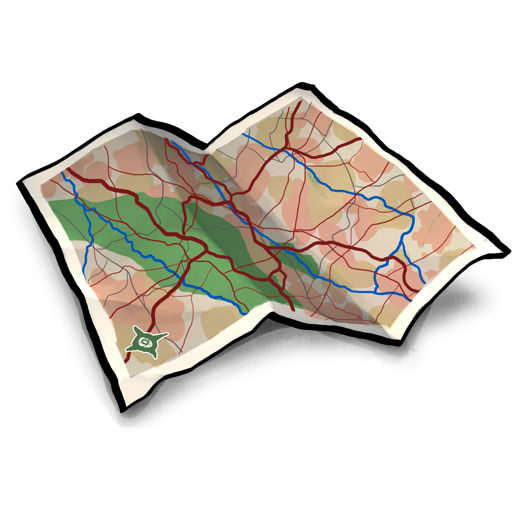
\includegraphics[height=.85em]{cv/loc.png}}
\newcommand{\phone}{
\includegraphics[height=.85em]{cv/phone.png}}

% Custom section spacing and formatting
\titleformat{\part}{\Huge\scshape\filcenter}{}{1em}{}
\titleformat{\section}{\Large\bf\raggedright}{}{1em}{}[{\titlerule[2pt]}]
\titlespacing{\section}{0pt}{3pt}{7pt}
\titleformat{\subsection}{\large\bfseries\centering}{}{0em}{\underline}%[\rule{3cm}{.2pt}]
\titlespacing{\subsection}{0pt}{7pt}{7pt}

% No indentation
\setlength{\parindent}{0in}

\begin{document}

\maketitle

\section{Basic Info}

\begin{minipage}[t]{.5\linewidth}
\begin{tabular}{rp{.75\linewidth}}
	\baselineskip=20pt
	\email{} :     & \href{mailto:mateusmelo1080p@protonmail.com}{mateusmelo1080p@protonmail.com}\\
	\www{} : &\href{https://mateusmelo.xyz}{https://mateusmelo.xyz}\\
	\loc{} : & Recife, Pernambuco, Brazil
\end{tabular}
\end{minipage}
\begin{minipage}[t]{.5\linewidth}
\begin{tabular}{rl}
	\gh{} : & \href{http://github.com/mateusgomes01}{github.com/mateusgomes01}\\
	\yt{} : &\href{https://www.youtube.com/channel/UCBAm2UMhkeX1P68CgHVJuOA}{mateusmelo}\\
	\phone{} : & +55 (81) 99128-2191
\end{tabular}
\end{minipage}

\begin{itemize}
\item Bachelor degree student in Computer Engineering at the \href{https://www.ufpe.br/cin}{Universidade Federal de Pernambuco \www}.
\end{itemize}

\section{Job Experience}
\entry{%feb/2020--today
	2021-Today}
	{Front-end web developer\href{https://www.liferay.com/home}{\www}}
	{\life}
	{Front-end software development and maintenance;

	Tools used: React; JavaScript; HTML \& CSS; git; virtual machines; vscode.
	
	\href{https://www.liferay.com/home}{https://www.liferay.com/home}}


\entry{%may/2020--feb/2021
	2020}
	{Full-stack web developer\href{https://europaycartoes.com.br}{\www}}
	{\euro}
	{Web app fullstack development and maintenance; IT support; creation and maintenance of spreadsheets and writen documents.
	
	Tools used: PHP + Laravel for back-end development and Vue.js for front-end; git; vscode; teamviewer; libre office.
	
	\href{https://europaycartoes.com.br/}{https://europaycartoes.com.br/}}

\entry{%aug/2019--nov/2019
	2019}
	{Siebel Junior developer\href{https://www.accenture.com/us-en}{\www}}
	{\acc}
	{Development and maintenance of Siebel features; Testing.
	
	Tools used: Siebel, VB6 for scripting, git, SVN, agile development, scrum.

	\href{https://www.accenture.com/us-en}{https://www.accenture.com/us-en}}
	
\section{Institutions}

\entry{2016--Today}
	{Bachelor Degree in Computer Engineering}
	{\ufpe, Recife, Pernambuco}
	%{Focusing on ...}

\entry{2011--2015}
	{Vocational Degree as an Electronics technician}
	{\ifpe, Recife, Pernambuco}
	%{Major in Syntax ...}

%\section{Classes Taught}

%\section{Presentations}

%\section{Guest Lectures}

\section{Languages}

\entry{Human}
	{Portuguese (native), English, some Japanese and some reading knowledge of Latin.}
	{}
	{}

\entry{Machine}
	{PHP, C, Python, JavaScript, VHDL/Verilog, Swift, SQL, Assembly and some basic BASH knowledge; markup languages including {\LaTeX}/{\XeTeX}, R Markdown, HTML, CSS/SASS.}
	{}
	{}

\section{Tools and Frameworks}

\subsection{Frameworks and programming tools}

React, Figma, Laravel, Vue.js, Bootstrap, RESTful APIs/http requests, nodeRED, Arduino, Git, MySQL Workbench, Terminal, Vim, Visual studio, RStudio, pandoc.
I've managed websites manually via ssh and vim using HTML + CSS and with tools such as Github Pages.

\subsection{Programs I'm Familiar With}

Audacity, GIMP, ffmpeg, youtube-dl, NNN, Ranger, Microsoft/Libre Office.

\subsection{General skills}

PCB Layout design, PLC Ladder programming, algorithms and data structures, programming tutoring, IoT.

\section{Projects}

\entry{2020}
	{http://MateusMelo.xyz \href{http://MateusMelo.xyz}{\www}}
	{My website}
	{Written from scratch. Modern traditional feel. I plan to make it better by generating the website offline with PHP and upload a static version of only HTML \& CSS.}
	
\entry{2019}
	{Hack-A-Truck project}
	{1 Month developing an iOS app with a team}
	{using swift, IoT + nodeRED and IBM Cloud technologies}
	
\entry{2019}
	{Programming Notes \href{https://mateusgomes01.github.io/project0/}{\www} \href{https://github.com/mateusgomes01/project0}{\gh}}
	{Based on Havard's CS50 lectures on web development \href{https://cs50.harvard.edu/web/2020/}{\www}}
	{Created mostly to put in practice what I learned in HTML \& CSS/SASS and also to practice the bootstrap framework.}

\entry{2019}
	{Online Resume/Portfolio \href{https://mateusgomes01.github.io/startbootstrap-resume/}{\www} \href{https://github.com/mateusgomes01/startbootstrap-resume}{\gh}}
	{Forked from startbootstrap-resume \href{https://github.com/StartBootstrap/startbootstrap-resume}{\gh}}
	{I try to keep it updated with my current activities, but I'll probably focus more on my personal webpage and keep this only as a portfolio to share some of my projects.}
	
\entry{2019}
	{tprm project \href{https://github.com/mateusgomes01/tprm-project}{\gh}}
	{A simple login interface in PHP + MySQL}
	{Made as a practice to learn the language and also as a project to be submitted for an internship vacancy at Bernhoeft \href{https://www.bernhoeft.com.br/}{https://www.bernhoeft.com.br/}.}
	
\entry{2015}
	{PWM analog circuit \href{https://www.youtube.com/watch?v=iVRAOyhpkvE}{\yt}}
	{Pulse Width Manipulation analog circuit} %Circuito analógico de ajuste PWM sincronizado com a rede elétrica
	{Synced with the electrical network. Done during my intership at \ifpe with guidance provided by professor Domingos Sávio.}

%\subsection{Other}

%My build of the the suckless \href{https://github.com/LukeSmithxyz/st}{simple terminal (st) \gh} with added homerow binds and small improvements.

%\section{Online Tutorials}

\section{Service}

\entry{2018-Today}
	{Private tutor of introduction to programming in C Language}
	{\ufpe}
	{ps: Not affiliated with the institution}

\entry{2017}
	{Graduate student mentor}
	{\ufpe}
	{Assisting in introduction to programming in C language classes}

\section{Hobbies}

Reading, songwriting, carpentry, free (i.e. libre) software, minimalism, survivalism

\section{References}

\begin{itemize}
	\item Email me \href{mailto:mateusmelo1080p@protonmail.com}{\email} with your interests in me and I'll refer you to someone who can vouch for me!

\end{itemize}

\end{document}
